\chapter{Ricerca per Interpolazione su Bucket e Ordinamento di Stringhe}
\label{chap:string-sorting-search}

\FloatBarrier
\section{Ricerca per Interpolazione Basata su Bucket}
\label{sec:bucket-interpolation-search}

La ricerca per interpolazione estende il principio della ricerca intuitiva impiegata nei dizionari o negli elenchi telefonici: conoscendo gli estremi numerici dei dati e assumendo una certa regolarit\`a distribuzionale, la posizione di un valore pu\`o essere stimata proiettando direttamente la chiave nell'intervallo dell'universo anzich\'e dividere ciecamente lo spazio a met\`a come avviene nella ricerca binaria standard.

\subsection{Definizione Formale del Modello e Partizione dell'Universo}
\label{subsec:modello-bucket-interpolation}

Sia dato un vettore ordinato $X[1 \dots n]$ composto da $n$ elementi interi distinti e disposti in ordine strettamente crescente:
\begin{equation}
  X = [x_1, x_2, \dots, x_n] \quad \text{con } x_i < x_{i+1} \quad \forall i \in \{1, \dots, n-1\}, \; x_i \in \mathbb{N}
\end{equation}

L'intervallo continuo discreto racchiuso tra l'elemento minimo e l'elemento massimo definisce l'\textbf{universo dei valori} $U = [x_1, x_n]$, la cui estensione complessiva (\textit{span}) \`e pari a:
\begin{equation}
  |U| = x_n - x_1 + 1
\end{equation}

Mentre la ricerca binaria standard garantisce un costo di $\mathcal{O}(\log_2 n)$ confronti operando unicamente sulla struttura degli indici, la \textbf{ricerca per interpolazione basata su bucket} sfrutta la cardinalit\`a dell'universo numerico per raggiungere un accesso diretto in tempo $\mathcal{O}(1)$ a una ristretta regione dell'array. 

A tal fine, l'universo $U$ viene suddiviso in $n$ partizioni contigue e disgiunte, denominate \textbf{bucket} ($B_1, B_2, \dots, B_n$), ciascuna avente un'ampiezza costante $b \in \mathbb{R}^+$ pari a:
\begin{equation}
  b = \frac{x_n - x_1 + 1}{n} = \frac{|U|}{n}
\end{equation}

Ciascun bucket generico $B_J$ (per $J \in \{1, \dots, n\}$) corrisponde all'intervallo semi-aperto a destra dei valori dell'universo:
\begin{equation}
  B_J = \left[ x_1 + (J-1)b, \; x_1 + Jb \right)
\end{equation}
con l'ultimo bucket $B_n = [x_1 + (n-1)b, \; x_1 + nb) = [x_1 + (n-1)b, \; x_n + 1)$, il quale copre e racchiude superiormente il valore massimo $x_n$.

\subsection{Struttura Dati Ausiliaria: Array degli Intervalli $I[J]$}
\label{subsec:struttura-array-intervalli}

Poich\'e i valori di $X$ possono presentare concentrazioni irregolari o lacune, la quantit\`a di elementi dell'array $X$ che ricadono all'interno di ciascun bucket $B_J$ non \`e a priori uniforme: alcuni bucket conterranno molteplici elementi di $X$, mentre altri risulteranno completamente vuoti.

Per consentire l'accesso immediato in tempo $\mathcal{O}(1)$ agli elementi di $X$ appartenenti a ciascun bucket, si costruisce durante la fase di pre-elaborazione un array ausiliario di delimitatori $I[1 \dots n]$:
\begin{itemize}
  \item Per ciascun bucket \textbf{non vuoto} $B_J$, la cella $I[J]$ memorizza una coppia di indici interi $\langle j_{\min}, j_{\max} \rangle$ che identificano il segmento contiguo in $X$ i cui elementi appartengono all'intervallo di $B_J$:
  \begin{equation}
    I[J] = \langle j_{\min}, j_{\max} \rangle \iff \forall k \in [j_{\min}, j_{\max}], \; X[k] \in B_J
  \end{equation}
  \item Se il bucket $B_J$ \`e \textbf{vuoto} (nessun elemento dell'array $X$ cade nell'intervallo $[x_1 + (J-1)b, x_1 + Jb)$), la voce viene contrassegnata con una coppia di valori sentinella:
  \begin{equation}
    I[J] = \langle -1, -1 \rangle
  \end{equation}
\end{itemize}

Lo spazio ausiliario richiesto dall'array $I$ \`e esattamente pari a $2n$ interi, ovvero $\mathcal{O}(n)$ parole di memoria, risultando asintoticamente lineare rispetto alla dimensione del vettore originario.

\begin{figure}[htbp]
\centering
\resizebox{\linewidth}{!}{%
\begin{tikzpicture}[
    >=Stealth,
    node distance=0.5cm,
    bkt/.style={draw=blue!80!black, thick, fill=blue!8, minimum height=0.9cm, font=\small, align=center},
    emptybkt/.style={draw=gray!50, dashed, fill=gray!8, minimum height=0.9cm, font=\small, align=center},
    arrnode/.style={draw=teal!80!black, thick, fill=teal!10, minimum height=0.8cm, minimum width=0.9cm, font=\small\bfseries},
    idxnode/.style={draw=orange!80!black, thick, fill=orange!10, minimum height=0.8cm, minimum width=1.4cm, font=\footnotesize\bfseries},
    arrline/.style={->, thick, blue!70!black},
    brace/.style={decorate, decoration={brace, amplitude=4pt, raise=2pt}, thick, teal!70!black}
]

  % Titoli a sinistra delle rispettive strutture (colonna dedicata, priva di collisioni con le frecce)
  \node[font=\bfseries\small, text=blue!90!black, anchor=east, align=right] at (-0.5, 3.0) {Partizione Universo $U$:\\{\scriptsize $[1, 36], \; n=12, \; b=3$}};
  \node[font=\bfseries\small, text=orange!90!black, anchor=east] at (-0.5, 1.4) {Array Intervalli $I[J]$:};
  \node[font=\bfseries\small, text=teal!90!black, anchor=east] at (-0.5, -0.6) {Array Dati Ordinato $X[1 \dots 12]$:};

  % Bucket visuali (primi 4 e ultimo)
  \node[bkt, minimum width=2.4cm] (b1) at (1.2, 3.0) {$B_1: [1, 4)$\\{\scriptsize $\{1, 2, 3\}$}};
  \node[emptybkt, minimum width=2.4cm] (b2) at (3.8, 3.0) {$B_2: [4, 7)$\\{\scriptsize \textit{Vuoto}}};
  \node[bkt, minimum width=2.4cm] (b3) at (6.4, 3.0) {$B_3: [7, 10)$\\{\scriptsize $\{8, 9\}$}};
  \node[emptybkt, minimum width=2.4cm] (b4) at (9.0, 3.0) {$B_4: [10, 13)$\\{\scriptsize \textit{Vuoto}}};
  \node[font=\large\bfseries] at (11.0, 3.0) {$\dots$};
  \node[bkt, minimum width=2.4cm] (b12) at (13.0, 3.0) {$B_{12}: [34, 37)$\\{\scriptsize $\{36\}$}};

  % Array I[J]
  \node[idxnode] (i1) at (1.2, 1.4) {$\langle 1, 3 \rangle$};
  \node[idxnode, draw=gray!60, fill=gray!10] (i2) at (3.8, 1.4) {$\langle -1, -1 \rangle$};
  \node[idxnode] (i3) at (6.4, 1.4) {$\langle 4, 5 \rangle$};
  \node[idxnode, draw=gray!60, fill=gray!10] (i4) at (9.0, 1.4) {$\langle -1, -1 \rangle$};
  \node[font=\large\bfseries] at (11.0, 1.4) {$\dots$};
  \node[idxnode] (i12) at (13.0, 1.4) {$\langle 12, 12 \rangle$};

  % Frecce tra Bucket e I[J]
  \draw[->, gray!70!black] (b1) -- (i1);
  \draw[->, gray!70!black] (b2) -- (i2);
  \draw[->, gray!70!black] (b3) -- (i3);
  \draw[->, gray!70!black] (b4) -- (i4);
  \draw[->, gray!70!black] (b12) -- (i12);

  % Array X[i]
  \node[arrnode] (x1) at (0.3, -0.6) {1};
  \node[arrnode] (x2) at (1.2, -0.6) {2};
  \node[arrnode] (x3) at (2.1, -0.6) {3};
  \node[arrnode] (x4) at (5.95, -0.6) {8};
  \node[arrnode] (x5) at (6.85, -0.6) {9};
  \node[font=\large\bfseries, text=teal!80!black] at (9.5, -0.6) {$\dots$};
  \node[arrnode] (x12) at (13.0, -0.6) {36};

  % Indici inferiori per X
  \node[font=\tiny, gray!80!black, below=1pt of x1] {$X[1]$};
  \node[font=\tiny, gray!80!black, below=1pt of x2] {$X[2]$};
  \node[font=\tiny, gray!80!black, below=1pt of x3] {$X[3]$};
  \node[font=\tiny, gray!80!black, below=1pt of x4] {$X[4]$};
  \node[font=\tiny, gray!80!black, below=1pt of x5] {$X[5]$};
  \node[font=\tiny, gray!80!black, below=1pt of x12] {$X[12]$};

  % Graffe orizzontali sopra X[1..3] e X[4..5]
  \draw[brace] (x1.north west) -- (x3.north east) node[midway, yshift=6pt] (br1) {};
  \draw[brace] (x4.north west) -- (x5.north east) node[midway, yshift=6pt] (br3) {};

  % Frecce verticali da I[J] verso il vertice delle graffe / cella di X
  \draw[arrline] (i1.south) -- (br1);
  \draw[arrline] (i3.south) -- (br3);
  \draw[arrline] (i12.south) -- (x12.north);

\end{tikzpicture}%
}
\caption{Architettura della Bucket Interpolation Search: partizione dell'universo numerico in bucket $B_J$ di ampiezza uniforme $b=3$, array ausiliario degli intervalli $I[J]$ con puntamento a graffa sui segmenti contigui del vettore ordinato dei dati $X$.}
\label{fig:bucket-interpolation-scheme}
\end{figure}

\subsection{Esempio Applicativo Completo}
\label{subsec:esempio-applicativo-bucket}

Si consideri un array ordinato composto da $n = 12$ elementi interi:
\begin{table}[H]
\centering
\small
\begin{tabular}{rcccccccccccc}
\toprule
\textbf{Indice $i$:} & 1 & 2 & 3 & 4 & 5 & 6 & 7 & 8 & 9 & 10 & 11 & 12 \\
\midrule
\textbf{$X[i]$:} & \textbf{1} & \textbf{2} & \textbf{3} & \textbf{8} & \textbf{9} & \textbf{17} & \textbf{19} & \textbf{20} & \textbf{28} & \textbf{30} & \textbf{32} & \textbf{36} \\
\bottomrule
\end{tabular}
\caption{Istanza didattica del vettore ordinato $X$ di $n=12$ elementi con distribuzione non uniforme.}
\label{tab:istanza-array-bucket}
\end{table}

\paragraph{Calcolo dei Parametri Strutturali:}
\begin{itemize}
  \item Estremi: $x_1 = 1$, $x_n = x_{12} = 36$.
  \item Estensione dell'universo: $|U| = 36 - 1 + 1 = 36$.
  \item Dimensione di ciascun bucket:
  \begin{equation}
    b = \frac{x_n - x_1 + 1}{n} = \frac{36 - 1 + 1}{12} = \frac{36}{12} = 3
  \end{equation}
\end{itemize}

I $12$ bucket partizionano l'intervallo continuo $[1, 36]$ a intervalli regolari di ampiezza $b = 3$. La Tabella~\ref{tab:bucket-mapping-trace} illustra la corrispondenza completa tra intervalli, elementi contenuti e voci dell'array $I[J]$.

\begin{table}[H]
\centering
\small
\resizebox{0.92\linewidth}{!}{%
\begin{tabular}{ccccc}
\toprule
\textbf{Bucket} & \textbf{Intervallo Numerico} & \textbf{Elementi in $X$} & \textbf{Indici in $X$} & \textbf{Array $I[J]$} \\
\midrule
$B_1$ & $[1, 4)$ & $\{1, 2, 3\}$ & Da $X[1]$ a $X[3]$ & $\langle 1, 3 \rangle$ \\
$B_2$ & $[4, 7)$ & $\emptyset$ & Nessuno & $\langle -1, -1 \rangle$ \\
$B_3$ & $[7, 10)$ & $\{8, 9\}$ & Da $X[4]$ a $X[5]$ & $\langle 4, 5 \rangle$ \\
$B_4$ & $[10, 13)$ & $\emptyset$ & Nessuno & $\langle -1, -1 \rangle$ \\
$B_5$ & $[13, 16)$ & $\emptyset$ & Nessuno & $\langle -1, -1 \rangle$ \\
$B_6$ & $[16, 19)$ & $\{17\}$ & Solo $X[6]$ & $\langle 6, 6 \rangle$ \\
$B_7$ & $[19, 22)$ & $\{19, 20\}$ & Da $X[7]$ a $X[8]$ & $\langle 7, 8 \rangle$ \\
$B_8$ & $[22, 25)$ & $\emptyset$ & Nessuno & $\langle -1, -1 \rangle$ \\
$B_9$ & $[25, 28)$ & $\emptyset$ & Nessuno & $\langle -1, -1 \rangle$ \\
$B_{10}$ & $[28, 31)$ & $\{28, 30\}$ & Da $X[9]$ a $X[10]$ & $\langle 9, 10 \rangle$ \\
$B_{11}$ & $[31, 34)$ & $\{32\}$ & Solo $X[11]$ & $\langle 11, 11 \rangle$ \\
$B_{12}$ & $[34, 37)$ & $\{36\}$ & Solo $X[12]$ & $\langle 12, 12 \rangle$ \\
\bottomrule
\end{tabular}%
}
\caption{Mappatura esaustiva dell'universo numerico per l'array didattico in esame.}
\label{tab:bucket-mapping-trace}
\end{table}

\subsection{Algoritmo di Ricerca e Tracciamento delle Operazioni}
\label{subsec:algoritmo-search-bucket}

Data una chiave interrogata $y \in [x_1, x_n]$, l'algoritmo di ricerca esegue la localizzazione in due stadi distinti:
\begin{enumerate}
  \item \textbf{Identificazione Diretta del Bucket in Tempo $\mathcal{O}(1)$:}
  Applicando la funzione di proiezione per interpolazione aritmetica, si determina l'indice $J$ del bucket di competenza:
  \begin{equation}
    J = \left\lfloor \frac{y - x_1}{b} \right\rfloor + 1
  \end{equation}
  \item \textbf{Verifica e Localizzazione Intra-Bucket:}
  Si consulta la voce $I[J]$ dell'array ausiliario:
  \begin{itemize}
    \item Se $I[J] = \langle -1, -1 \rangle$, il bucket \`e vuoto; si conclude immediatamente che $y \notin X$ in tempo $\mathcal{O}(1)$, senza compiere alcun accesso alla memoria dell'array $X$.
    \item Se $I[J] = \langle j_{\min}, j_{\max} \rangle \neq \langle -1, -1 \rangle$, l'elemento $y$ pu\`o trovarsi esclusivamente all'interno del segmento $X[j_{\min} \dots j_{\max}]$. Si esegue una ricerca binaria ristretta unicamente a questo intervallo locale di dimensione $|B_J| = j_{\max} - j_{\min} + 1$.
  \end{itemize}
\end{enumerate}

\begin{algorithm}[H]
\caption{Bucket Interpolation Search}
\label{algo:bucket-search}
\KwInput{Vettore ordinato $X[1 \dots n]$, array intervalli $I[1 \dots n]$, estremo inferiore $x_1$, ampiezza bucket $b$, chiave cercata $y$}
\KwOutput{Indice $pos$ tale che $X[pos] = y$, oppure $-1$ se assente}

\BlankLine
\tcp{Verifica confini dell'universo}
\If{$y < x_1$ \textbf{oppure} $y > x_n$}{
    \Return $-1$\;
}

\BlankLine
\tcp{Stadio 1: Proiezione aritmetica in tempo $O(1)$}
$J \leftarrow \min\left(n, \; \left\lfloor \frac{y - x_1}{b} \right\rfloor + 1 \right)$\;

\BlankLine
\tcp{Stadio 2: Ispezione della voce ausiliaria $I[J]$}
\If{$I[J] = \langle -1, -1 \rangle$}{
    \Return $-1$ \tcp*{Terminazione immediata: bucket vuoto}
}

$\langle j_{\min}, j_{\max} \rangle \leftarrow I[J]$\;
\Return $\text{BinarySearch}(X, \; \text{key} = y, \; \text{low} = j_{\min}, \; \text{high} = j_{\max})$\;
\end{algorithm}

\paragraph{Esempio di Traccia 1: Ricerca di Chiave Presente ($y = 9$):}
\begin{enumerate}
  \item Calcolo del bucket:
  \begin{equation}
    J = \left\lfloor \frac{9 - 1}{3} \right\rfloor + 1 = \left\lfloor \frac{8}{3} \right\rfloor + 1 = 2 + 1 = 3
  \end{equation}
  Costo: un'operazione aritmetica elementare in tempo $\mathcal{O}(1)$.
  \item Ispezione di $I[3]$: si riscontra $I[3] = \langle 4, 5 \rangle \neq \langle -1, -1 \rangle$.
  \item Ricerca binaria ristretta al sotto-array $X[4 \dots 5] = [8, 9]$:
  \begin{equation}
    \text{Costo: } \mathcal{O}(\log_2 |B_3|) = \mathcal{O}(\log_2 2) = 1 \text{ confronto}
  \end{equation}
  L'elemento viene identificato alla posizione $X[5] = 9$.
\end{enumerate}

\paragraph{Esempio di Traccia 2: Ricerca di Chiave Assente ($y = 5$):}
\begin{enumerate}
  \item Calcolo del bucket:
  \begin{equation}
    J = \left\lfloor \frac{5 - 1}{3} \right\rfloor + 1 = \left\lfloor \frac{4}{3} \right\rfloor + 1 = 1 + 1 = 2
  \end{equation}
  \item Ispezione di $I[2]$: si riscontra $I[2] = \langle -1, -1 \rangle$.
  \item L'algoritmo termina immediatamente restituendo $-1$ in tempo $\mathcal{O}(1)$, senza effettuare alcuna comparazione nell'array dei dati $X$.
\end{enumerate}

\subsection{Analisi della Complessità: Approccio Data-Aware e Parametro $\Delta$}
\label{subsec:analisi-complessita-data-aware}

La complessit\`a temporale dell'algoritmo di ricerca dipende dalla cardinalit\`a $|B_J|$ del bucket indirizzato dalla chiave $y$:
\begin{equation}
  T(n) = \mathcal{O}(1) + \mathcal{O}(\log_2 |B_J|) \quad \text{con } 0 \le |B_J| \le b
\end{equation}

Nel caso peggiore degenere (tutti gli $n$ elementi concentrati in un unico intervallo di ampiezza $b$), si avrebbe $|B_J| = n$, riconducendosi al costo della ricerca binaria standard $\mathcal{O}(\log_2 n)$. Tuttavia, sviluppando un'analisi \textbf{Data-Aware} (sensibile alla struttura intrinseca dei dati), \`e possibile esprimere la complessit\`a in funzione della dispersione dei divari tra elementi contigui.

\begin{definition}[Gap tra Elementi Consecutivi]
Dato il vettore ordinato $X[1 \dots n]$, si definisce \textbf{gap} $i$-esimo la differenza scalare tra due elementi consecutivi:
\begin{equation}
  g_i = x_i - x_{i-1} \quad \forall i \in \{2, \dots, n\}
\end{equation}
\end{definition}

\begin{lemma}[Limite Inferiore per il Gap Massimo]
\label{lem:gap-massimo}
Dato un vettore ordinato di $n$ elementi con universo $U = [x_1, x_n]$ e ampiezza di bucket $b = \frac{x_n - x_1 + 1}{n}$, il massimo divario tra elementi adiacenti soddisfa la disuguaglianza:
\begin{equation}
  \max_{i=2 \dots n} g_i \ge b
\end{equation}
\end{lemma}

\begin{proof}
La somma di tutti gli $n-1$ divari contigui costituisce una somma telescopica la cui risultante \`e la dispersione complessiva dell'array:
\begin{equation}
  \sum_{i=2}^n g_i = \sum_{i=2}^n (x_i - x_{i-1}) = x_n - x_1
\end{equation}
Il divario medio aritmetico tra elementi consecutivi \`e pertanto:
\begin{equation}
  \bar{g} = \frac{\sum_{i=2}^n g_i}{n - 1} = \frac{x_n - x_1}{n - 1}
\end{equation}
Poich\'e il valore massimo di un insieme finito di numeri reali non pu\`o mai essere inferiore alla rispettiva media aritmetica, si ha necessariamente:
\begin{equation}
  \max_{i=2 \dots n} g_i \ge \bar{g} = \frac{x_n - x_1}{n - 1}
\end{equation}
Osservando che $n - 1 < n$ e che $x_n - x_1 < x_n - x_1 + 1$, vale la catena di disuguaglianze:
\begin{equation}
  \frac{x_n - x_1}{n - 1} \ge \frac{x_n - x_1 + 1}{n} = b
\end{equation}
Confrontando i due membri estremi si ottiene la tesi:
\begin{equation}
  \max_{i=2 \dots n} g_i \ge b
\end{equation}
\end{proof}

\begin{theorem}[Limite Superiore alla Dimensione del Bucket e Complessit\`a Data-Aware]
\label{thm:complessita-data-aware}
Sia $\Delta$ il \textbf{rapporto di dispersione dei gap} (\textit{gap ratio}) definito da:
\begin{equation}
  \Delta = \frac{\displaystyle\max_{i=2 \dots n} (x_i - x_{i-1})}{\displaystyle\min_{i=2 \dots n} (x_i - x_{i-1})} = \frac{\max g}{\min g}
\end{equation}
La cardinalit\`a di qualsiasi bucket $B_J$ \`e limitata superiormente da $|B_J| \le \Delta$, e la complessit\`a temporale della ricerca soddisfa:
\begin{equation}
  T(n) = \mathcal{O}(\log_2 \Delta)
\end{equation}
\end{theorem}

\begin{proof}
Ciascun bucket $B_J$ copre un intervallo di ampiezza $b$. Due elementi distinti dell'array $X$ che ricadono all'interno del medesimo bucket $B_J$ devono distare tra loro almeno una quantit\`a pari al divario minimo presente nell'intera sequenza, ovvero $\min_{i=2 \dots n} g_i$.

Di conseguenza, il numero massimo di elementi distinti che possono coesistere in un intervallo continuo di ampiezza $b$ \`e limitato superiormente dal rapporto:
\begin{equation}
  |B_J| \le \frac{b}{\min_{i=2 \dots n} g_i}
\end{equation}
Applicando il Lemma~\ref{lem:gap-massimo}, per cui $b \le \max_{i=2 \dots n} g_i$, si ottiene direttamente:
\begin{equation}
  |B_J| \le \frac{\max_{i=2 \dots n} g_i}{\min_{i=2 \dots n} g_i} = \Delta
\end{equation}
Poich\'e la ricerca locale all'interno del bucket viene eseguita mediante ricerca binaria sul segmento di dimensione $|B_J|$, il costo temporale complessivo ammonta a:
\begin{equation}
  T(n) = \mathcal{O}(1) + \mathcal{O}(\log_2 |B_J|) \le \mathcal{O}(\log_2 \Delta)
\end{equation}
\end{proof}

\paragraph{Interpretazione Ingegneristica e Casi Notevoli:}
\begin{itemize}
  \item \textbf{Distribuzione Uniforme ($\Delta = \mathcal{O}(1)$):} Se le chiavi sono distanziate in modo omogeneo, il rapporto tra il divario massimo e il divario minimo \`e limitato da una costante. Ne consegue che ogni bucket contiene al pi\`u un numero costante di elementi ($|B_J| \le c$), e la ricerca termina in tempo ottimo costante:
  \begin{equation}
    T(n) = \mathcal{O}(\log_2 \mathcal{O}(1)) = \mathcal{O}(1)
  \end{equation}
  \item \textbf{Resilienza Logaritmica:} All'aumentare dell'asimmetria distribuzionale, il parametro $\Delta$ cresce. Tuttavia, poich\'e il parametro entra sotto l'operatore logaritmo, l'impatto sul tempo di ricerca risulta fortemente smorzato: persino con un rapporto di sbilanciamento enorme $\Delta = 10^6$, sono necessari meno di $20$ confronti locali.
  \item \textbf{Comportamento Probabilistico su Dati Casuali:} Se le $n$ chiavi sono generate come variabili aleatorie indipendenti e identicamente distribuite (i.i.d.) secondo una distribuzione uniforme continua sull'intervallo $[x_1, x_n]$, la teoria probabilistica dell'occupancy problem dimostra che la cardinalit\`a massima di un bucket soddisfa:
  \begin{equation}
    |B_J| = \mathcal{O}\left( \log_2^2 n \right) \quad \text{con alta probabilit\`a (w.h.p.)}
  \end{equation}
  Sostituendo tale valore nell'espressione della complessit\`a locale, si ottiene un costo atteso eccezionalmente basso:
  \begin{equation}
    T(n) = \mathcal{O}\left( \log_2 \left( \log_2^2 n \right) \right) = \mathcal{O}\left( 2 \log_2 \log_2 n \right) = \mathcal{O}(\log_2 \log_2 n)
  \end{equation}
  risultato in perfetto accordo con la teoria classica della ricerca per interpolazione di Perl, Itai e Avni~\cite{perl1978}.
\end{itemize}

\FloatBarrier
\section{Ordinamento di Stringhe e Analisi del Limite Inferiore}
\label{sec:string-sorting-lower-bound}

Quando le chiavi da ordinare non sono scalari compatti ma sequenze di caratteri a lunghezza variabile, il costo del confronto tra elementi cessa di essere unitario ($\mathcal{O}(1)$). In questa sezione formalizziamo il modello computazionale per le stringhe, evidenziamo i colli di bottiglia del Quicksort convenzionale e deriviamo il limite inferiore teorico del problema.

\subsection{Modello di Calcolo e Notazione}
\label{subsec:modello-string-sorting}

Sia dato un insieme $S$ composto da $n$ stringhe definite sopra un alfabeto finito e totalmente ordinato $\Sigma$:
\begin{equation}
  S = \{s_1, s_2, \dots, s_n\}
\end{equation}

I parametri dimensionali che governano il problema sono:
\begin{itemize}
  \item $n = |S|$: numero totale di stringhe appartenenti all'insieme.
  \item $N = \sum_{j=1}^n |s_j|$: lunghezza cumulativa (numero totale di caratteri) di tutte le stringhe in $S$.
  \item $\sigma = |\Sigma|$: dimensione (cardinalit\`a) dell'alfabeto dei simboli.
  \item $\bar{L} = \frac{N}{n}$: lunghezza media delle stringhe nella collezione.
\end{itemize}

Nel modello di memoria reale, l'insieme $S$ \`e rappresentato mediante un \textbf{array di puntatori} $S[1 \dots n]$. Ciascuna cella $S[k]$ memorizza un indirizzo di memoria (a 64 bit) che punta all'area contigua nell'heap dove risiedono i caratteri della stringa $s_k$, terminata dal carattere nullo speciale (\texttt{'\textbackslash0'}), come illustrato in \autoref{fig:string-memory-layout}.

\begin{figure}[htbp]
\centering
\begin{tikzpicture}[
    >=Stealth,
    ptr/.style={draw=black!75, thick, fill=blue!10, minimum height=0.7cm, minimum width=1.5cm, font=\small\ttfamily},
    charbox/.style={draw=teal!80!black, thick, fill=teal!10, minimum height=0.65cm, minimum width=0.65cm, font=\small\ttfamily},
    nullbox/.style={draw=gray!70, thick, fill=gray!20, minimum height=0.65cm, minimum width=0.65cm, font=\small\ttfamily\color{gray!80!black}},
    arr/.style={->, thick, blue!80!black}
]

  % Array di puntatori
  \node[font=\bfseries\small, text=blue!90!black, anchor=south] at (0, 2.3) {Array Puntatori $S$:};
  \node[ptr] (p1) at (0, 1.8) {S[1]};
  \node[ptr] (p2) at (0, 1.0) {S[2]};
  \node[ptr] (p3) at (0, 0.2) {S[3]};
  \node[ptr] (pn) at (0, -1.0) {S[n]};
  \draw[dotted, thick] (0, -0.3) -- (0, -0.6);

  % Stringhe nell'heap
  \node[font=\bfseries\small, text=teal!90!black, anchor=south] at (6.0, 2.3) {Buffer di Caratteri in Heap:};

  % S[1] -> "PAOLO\0"
  \node[charbox] (c11) at (4.0, 1.8) {P};
  \node[charbox] (c12) at (4.65, 1.8) {A};
  \node[charbox] (c13) at (5.3, 1.8) {O};
  \node[charbox] (c14) at (5.95, 1.8) {L};
  \node[charbox] (c15) at (6.6, 1.8) {O};
  \node[nullbox] (c16) at (7.25, 1.8) {\textbackslash 0};
  \draw[arr] (p1.east) -- (c11.west);

  % S[2] -> "BOO\0"
  \node[charbox] (c21) at (4.0, 1.0) {B};
  \node[charbox] (c22) at (4.65, 1.0) {O};
  \node[charbox] (c23) at (5.3, 1.0) {O};
  \node[nullbox] (c24) at (5.95, 1.0) {\textbackslash 0};
  \draw[arr] (p2.east) -- (c21.west);

  % S[3] -> "BOX\0"
  \node[charbox] (c31) at (4.0, 0.2) {B};
  \node[charbox] (c32) at (4.65, 0.2) {O};
  \node[charbox] (c33) at (5.3, 0.2) {X};
  \node[nullbox] (c34) at (5.95, 0.2) {\textbackslash 0};
  \draw[arr] (p3.east) -- (c31.west);

  % S[n] -> "AC\0"
  \node[charbox] (cn1) at (4.0, -1.0) {A};
  \node[charbox] (cn2) at (4.65, -1.0) {C};
  \node[nullbox] (cn3) at (5.3, -1.0) {\textbackslash 0};
  \draw[arr] (pn.east) -- (cn1.west);

\end{tikzpicture}
\caption{Rappresentazione standard in memoria per collezioni di stringhe: array di puntatori contiguo e buffer di caratteri a lunghezza variabile sparsi nell'heap.}
\label{fig:string-memory-layout}
\end{figure}

\subsection{Limiti del Quicksort Classico su Stringhe}
\label{subsec:limiti-quicksort-classico}

Un approccio ingenuo al problema consiste nell'invocare l'algoritmo Quicksort tradizionale sull'array di puntatori $S$, delegando il confronto d'ordine a una funzione di comparazione lessicografica a due vie (quale \texttt{strcmp} in linguaggio C):
\begin{equation}
  \text{qSORT}(S, \; 1, \; n, \; \text{cmp} = \texttt{strcmp})
\end{equation}

Questa architettura manifesta due gravi inefficienze strutturali:

\begin{enumerate}
  \item \textbf{Costo Computazionale Super-Lineare dei Confronti:}
  Il Quicksort standard esegue $\mathcal{O}(n \log_2 n)$ confronti tra elementi. Mentre per i tipi primitivi ciascuna comparazione costa $\mathcal{O}(1)$ cicli macchina, la funzione \texttt{strcmp} tra due stringhe $s_a, s_b$ deve scorrere i caratteri in avanti partendo dalla prima posizione sino a incontrare il primo simbolo disuguale. Nel caso medio, il confronto richiede un numero di operazioni proporzionale alla lunghezza del prefisso comune, che pu\`o estendersi fino all'intera lunghezza media $\bar{L} = \frac{N}{n}$. 
  
  Moltiplicando il numero di confronti per il costo medio di ciascuna comparazione si ottiene:
  \begin{equation}
    T(n, N) = \mathcal{O}(n \log_2 n) \cdot \mathcal{O}\left( \frac{N}{n} \right) = \mathcal{O}(N \log_2 n)
  \end{equation}
  Tale costo \`e intrinsecamente ridondante: se un gruppo di stringhe condivide un lungo prefisso comune (ad esempio 50 caratteri identici), tali primi 50 caratteri vengono ri-confrontati da capo a ogni singolo livello di profondit\`a dell'albero di ricorsione del Quicksort.
  
  \item \textbf{Assenza di Localit\`a di Riferimento (\textit{Poor Cache Locality}):}
  Sebbene l'array dei puntatori $S$ sia allocato in un blocco contiguo di memoria, i buffer contenenti i caratteri delle stringhe risiedono in regioni arbitrarie dell'heap. A ogni confronto eseguito da \texttt{strcmp}, la CPU deve dereferenziare due puntatori distanti, generando continui salti casuali nella memoria virtuale. Ci\`o causa un numero elevatissimo di \textbf{cache miss} sia nella gerarchia L1/L2/L3 sia nel TLB (\textit{Translation Lookaside Buffer}), degradando pesantemente il throughput effettivo del processore.
\end{enumerate}

\subsection{Analisi del Limite Inferiore: Lower Bound per lo String Sorting}
\label{subsec:lower-bound-analysis}

Per determinare l'efficienza teorica di qualsiasi algoritmo di ordinamento basato su confronti di singoli caratteri (\textit{atomic character comparisons}), decomponiamo l'attivit\`a computazionale necessaria in due componenti indipendenti e non sovrapposte.

\paragraph{Componente 1: Ordinamento Combinatorio delle Permutazioni.}
Anche nell'ipotesi ideale in cui tutte le $n$ stringhe dell'insieme $S$ possiedano caratteri iniziali reciprocamente distinti (distinguibili al passo $1$), l'algoritmo deve comunque determinare l'unica permutazione ordinata tra le $n!$ possibili disposizioni dell'insieme. 

In base al classico modello dell'albero di decisione basato su confronti binari:
\begin{equation}
  \text{Altezza dell'albero} \ge \log_2(n!) = \Omega(n \log_2 n)
\end{equation}
Sono quindi strettamente necessari almeno $\Omega(n \log_2 n)$ confronti atomici tra caratteri.

\paragraph{Componente 2: Ispezione dei Prefissi Distinguibili ($d_s$) e LCP.}
In presenza di stringhe che condividono prefissi identici, non \`e sufficiente ordinare le stringhe come entit\`a astratte: l'algoritmo deve necessariamente scendere lungo i caratteri condivisi per identificare il primo simbolo discriminante.

\begin{definition}[Longest Common Prefix --- LCP]
Date due stringhe $s_a, s_b \in \Sigma^*$, si definisce $\text{LCP}(s_a, s_b)$ la lunghezza del pi\`u lungo prefisso comune identico condiviso da entrambe:
\begin{equation}
  \text{LCP}(s_a, s_b) = \max \left\{ \ell \ge 0 \;\middle|\; s_a[1 \dots \ell] = s_b[1 \dots \ell] \right\}
\end{equation}
\end{definition}

\begin{definition}[Prefisso Distinguibile $d_s$]
Data una stringa $s \in S$ e considerato l'ordinamento lessicografico globale di $S$, si definisce \textbf{prefisso distinguibile} $d_s$ il numero minimo di caratteri di $s$ che qualsiasi algoritmo corretto deve obbligatoriamente esaminare per distinguerla in modo univoco sia dal suo predecessore immediato ($\text{pred}(s)$) sia dal suo successore immediato ($\text{succ}(s)$) nella sequenza ordinata:
\begin{equation}
  d_s = 1 + \max \left( \text{LCP}(s, \; \text{pred}(s)), \; \text{LCP}(s, \; \text{succ}(s)) \right)
\end{equation}
ponendo per convenzione $\text{LCP}(s_1, \text{pred}(s_1)) = 0$ per la prima stringa e $\text{LCP}(s_n, \text{succ}(s_n)) = 0$ per l'ultima.
\end{definition}

Si definisce quindi la somma dei prefissi distinguibili su tutte le $n$ stringhe dell'insieme:
\begin{equation}
  d = \sum_{s \in S} d_s
\end{equation}

\begin{figure}[htbp]
\centering
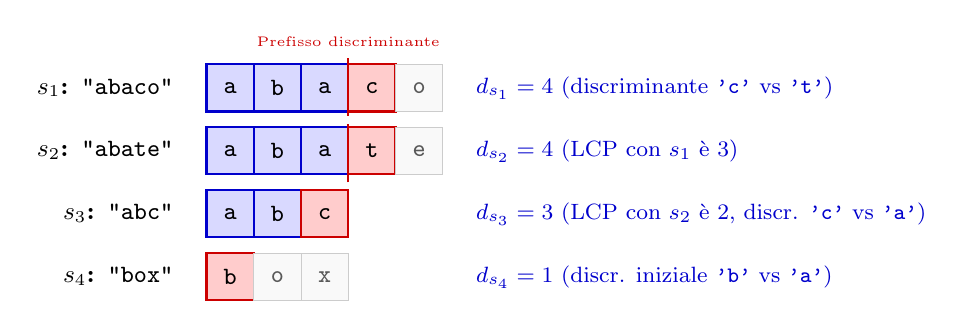
\begin{tikzpicture}[
    char/.style={draw=black!70, thick, minimum size=0.6cm, font=\ttfamily\small},
    lcpchar/.style={draw=blue!80!black, thick, fill=blue!15, minimum size=0.6cm, font=\ttfamily\small\bfseries},
    diffchar/.style={draw=red!80!black, thick, fill=red!20, minimum size=0.6cm, font=\ttfamily\small\bfseries},
    ignchar/.style={draw=gray!40, fill=gray!5, minimum size=0.6cm, font=\ttfamily\small\color{gray!70!black}}
]

  % Stringa 1: abaco
  \node[font=\small\bfseries, anchor=east] at (-0.3, 2.4) {$s_1$: \texttt{"abaco"}};
  \node[lcpchar] at (0.3, 2.4) {a};
  \node[lcpchar] at (0.9, 2.4) {b};
  \node[lcpchar] at (1.5, 2.4) {a};
  \node[diffchar] at (2.1, 2.4) {c};
  \node[ignchar] at (2.7, 2.4) {o};
  \node[font=\footnotesize, anchor=west, text=blue!80!black] at (3.3, 2.4) {$\implies d_{s_1} = 4$ (discriminante \texttt{'c'} vs \texttt{'t'})};

  % Stringa 2: abate
  \node[font=\small\bfseries, anchor=east] at (-0.3, 1.6) {$s_2$: \texttt{"abate"}};
  \node[lcpchar] at (0.3, 1.6) {a};
  \node[lcpchar] at (0.9, 1.6) {b};
  \node[lcpchar] at (1.5, 1.6) {a};
  \node[diffchar] at (2.1, 1.6) {t};
  \node[ignchar] at (2.7, 1.6) {e};
  \node[font=\footnotesize, anchor=west, text=blue!80!black] at (3.3, 1.6) {$\implies d_{s_2} = 4$ (LCP con $s_1$ \`e 3)};

  % Stringa 3: abc
  \node[font=\small\bfseries, anchor=east] at (-0.3, 0.8) {$s_3$: \texttt{"abc"}};
  \node[lcpchar] at (0.3, 0.8) {a};
  \node[lcpchar] at (0.9, 0.8) {b};
  \node[diffchar] at (1.5, 0.8) {c};
  \node[font=\footnotesize, anchor=west, text=blue!80!black] at (3.3, 0.8) {$\implies d_{s_3} = 3$ (LCP con $s_2$ \`e 2, discr. \texttt{'c'} vs \texttt{'a'})};

  % Stringa 4: box
  \node[font=\small\bfseries, anchor=east] at (-0.3, 0.0) {$s_4$: \texttt{"box"}};
  \node[diffchar] at (0.3, 0.0) {b};
  \node[ignchar] at (0.9, 0.0) {o};
  \node[ignchar] at (1.5, 0.0) {x};
  \node[font=\footnotesize, anchor=west, text=blue!80!black] at (3.3, 0.0) {$\implies d_{s_4} = 1$ (discr. iniziale \texttt{'b'} vs \texttt{'a'})};

  % Linee di demarcazione LCP
  \draw[dashed, red!80!black, thick] (1.8, 1.2) -- (1.8, 2.8);
  \node[font=\tiny, text=red!80!black, above] at (1.8, 2.8) {Prefisso discriminante};

\end{tikzpicture}
\caption{Visualizzazione dei prefissi distinguibili $d_s$ su stringhe ordinate lessicograficamente: le celle azzurre rappresentano i caratteri condivisi (LCP), le celle rosse denotano il carattere discriminante obbligatorio ($d_s$), mentre le celle grigie non necessitano di ispezione.}
\label{fig:distinguishable-prefixes}
\end{figure}

Nessun algoritmo di ordinamento pu\`o esimersi dall'ispezionare ciascuno dei $d_s$ caratteri per ogni stringa $s \in S$: qualora un carattere compreso nel prefisso distinguibile non venisse letto, l'ordinamento relativo tra $s$ e i suoi vicini lessicografici rimarrebbe indecidibile. Ne consegue che sono strettamente necessarie almeno $\Omega(d)$ operazioni atomiche di lettura e confronto.

\begin{theorem}[Limite Inferiore per lo String Sorting]
\label{thm:lower-bound-string-sorting}
Dato un insieme di $n$ stringhe $S$ con somma dei prefissi distinguibili $d = \sum_{s \in S} d_s$, la complessit\`a di qualsiasi algoritmo di ordinamento basato su confronti atomici tra caratteri soddisfa il limite inferiore:
\begin{equation}
  \Omega(d + n \log_2 n) \quad \text{confronti di caratteri}
\end{equation}
\end{theorem}

\begin{proof}
La dimostrazione discende direttamente dall'indipendenza delle due componenti necessarie:
\begin{enumerate}
  \item Per distinguere ogni stringa dai suoi vicini immediati, l'algoritmo deve ispezionare tutti i caratteri del prefisso distinguibile, imponendo un numero di letture pari ad almeno $\Omega(d)$.
  \item Per identificare la corretta permutazione tra le $n$ stringhe indipendentemente dalla lunghezza dei caratteri discriminanti, l'albero di decisione impone almeno $\Omega(\log_2(n!)) = \Omega(n \log_2 n)$ diramazioni binarie.
\end{enumerate}
Poich\'e le due richieste computazionali devono essere soddisfatte contemporaneamente, la complessit\`a complessiva \`e dominata dal termine congiunto $\Omega(d + n \log_2 n)$.
\end{proof}

\FloatBarrier
\section{Multi-Key Quicksort: 3-Way Radix Quicksort}
\label{sec:multikey-quicksort}

L'algoritmo \textbf{Multi-Key Quicksort} (noto anche come algoritmo di Bentley-Sedgewick o 3-Way Radix Quicksort~\cite{bentley1997}) risolve in modo elegante le inefficienze del Quicksort classico combinando il partizionamento a tre vie di Dijkstra per chiavi duplicate con la scansione progressiva per singoli caratteri tipica del Radix Sort.

\subsection{Principio di Funzionamento e Invariante Fondamentale}
\label{subsec:principio-invariante-multikey}

L'algoritmo opera ricorsivamente su una coppia $(R, i)$:
\begin{itemize}
  \item $R \subseteq S$: sottoinsieme corrente di stringhe da ordinare.
  \item $i \in \mathbb{N}^+$: indice posizionale (1-based) del carattere corrente da confrontare.
\end{itemize}

\begin{alertblock}{Invariante Fondamentale del Multi-Key Quicksort}
All'atto della chiamata ricorsiva $\text{MKQ}(R, i)$, tutte le stringhe appartenenti al sottoinsieme $R$ condividono un prefisso comune identico di lunghezza esattamente pari a $i - 1$ caratteri:
\begin{equation}
  \forall s_a, s_b \in R, \quad s_a[1 \dots i-1] = s_b[1 \dots i-1]
\end{equation}
\end{alertblock}

Questo invariante garantisce che i primi $i-1$ caratteri non debbano \textbf{mai pi\`u essere ri-confrontati}, abbattendo alla radice la ridondanza di \texttt{strcmp}.

\subsection{Formalizzazione dell'Algoritmo ed Esecuzione Ricorsiva}
\label{subsec:formalizzazione-algoritmo-mkq}

Dato il sottoinsieme di stringhe $R$ e l'indice $i$:
\begin{enumerate}
  \item \textbf{Caso Base:} Se $|R| \le 1$, l'insieme \`e banalmente ordinato: restituisci $R$.
  \item \textbf{Selezione del Pivot:} Si sceglie una stringa di pivot $p \in R$ (ad esempio casualmente, o mediante la mediana di un piccolo campione) e si estrae il suo $i$-esimo carattere $p[i]$.
  \item \textbf{Partizionamento a Tre Vie (3-Way Partitioning):} L'insieme $R$ viene partizionato rispetto al carattere $p[i]$ in tre sottoinsiemi disgiunti:
  \begin{align}
    R_< &= \{ s \in R \mid s[i] < p[i] \} \\
    R_= &= \{ s \in R \mid s[i] = p[i] \} \\
    R_> &= \{ s \in R \mid s[i] > p[i] \}
  \end{align}
  \item \textbf{Chiamate Ricorsive e Regola di Avanzamento dell'Indice $i$:}
  \begin{itemize}
    \item $A = \text{MKQ}(R_<, \; i)$: le stringhe in $R_<$ hanno $s[i] < p[i]$, ma possono differire tra loro alla posizione $i$. L'indice $i$ \textbf{rimane invariato}.
    \item $B = \text{MKQ}(R_=, \; i + 1)$: tutte le stringhe in $R_=$ possiedono esattamente lo stesso carattere $p[i]$ alla posizione $i$. Avendo validato la concordanza su tale simbolo, l'invariante si estende a $i$ caratteri e l'indice avanza: \textbf{$i \leftarrow i + 1$}.
    \item $C = \text{MKQ}(R_>, \; i)$: le stringhe in $R_>$ hanno $s[i] > p[i]$; l'indice $i$ \textbf{rimane invariato}.
  \end{itemize}
  \item \textbf{Composizione del Risultato:} Si restituisce la concatenazione ordinata:
  \begin{equation}
    \text{MKQ}(R, i) = A \cdot B \cdot C
  \end{equation}
\end{enumerate}

\begin{algorithm}[H]
\caption{Multi-Key Quicksort ($\text{MKQ}(R, i)$)}
\label{algo:multikey-quicksort}
\KwInput{Insieme di stringhe $R \subseteq S$, indice del carattere corrente $i$}
\KwOutput{Insieme $R$ ordinato lessicograficamente}

\BlankLine
\If{$|R| \le 1$}{
    \Return $R$\;
}

\BlankLine
\tcp{Selezione del pivot e del carattere discriminante}
Scegli una stringa pivot $p \in R$\;
$c \leftarrow p[i]$\;

\BlankLine
\tcp{Partizionamento ternario in-place}
$R_< \leftarrow \{ s \in R \mid s[i] < c \}$\;
$R_= \leftarrow \{ s \in R \mid s[i] = c \}$\;
$R_> \leftarrow \{ s \in R \mid s[i] > c \}$\;

\BlankLine
\tcp{Rami ricorsivi: solo il ramo centrale avanza l'indice $i$}
$A \leftarrow \text{MKQ}(R_<, \; i)$\;
$B \leftarrow \text{MKQ}(R_=, \; i + 1)$\;
$C \leftarrow \text{MKQ}(R_>, \; i)$\;

\BlankLine
\Return $A \cdot B \cdot C$\;
\end{algorithm}

\begin{figure}[htbp]
\centering
\resizebox{0.95\linewidth}{!}{%
\begin{tikzpicture}[
    >=Stealth,
    node distance=1.0cm and 1.5cm,
    mainbox/.style={draw=blue!80!black, thick, fill=blue!8, rounded corners=3pt, minimum width=3.2cm, minimum height=1.0cm, align=center, font=\small},
    branchbox/.style={draw=teal!80!black, thick, fill=teal!8, rounded corners=3pt, minimum width=2.8cm, minimum height=1.0cm, align=center, font=\small},
    advbox/.style={draw=orange!80!black, thick, fill=orange!10, rounded corners=3pt, minimum width=3.0cm, minimum height=1.0cm, align=center, font=\small},
    arr/.style={->, thick, draw=black!75}
]

  % Nodo radice
  \node[mainbox] (root) {$\text{MKQ}(R, i)$\\{\footnotesize Pivot: $p[i]$}};

  % Nodi figli
  \node[branchbox, below left=1.2cm and 1.8cm of root] (left) {$R_< = \{s \in R \mid s[i] < p[i]\}$\\\textbf{$\text{MKQ}(R_<, \; i)$}\\{\footnotesize (indice $i$ invariato)}};
  \node[advbox, below=1.2cm of root] (mid) {$R_= = \{s \in R \mid s[i] = p[i]\}$\\\textbf{$\text{MKQ}(R_=, \; i + 1)$}\\{\footnotesize \textbf{Avanza: $i \leftarrow i + 1$}}};
  \node[branchbox, below right=1.2cm and 1.8cm of root] (right) {$R_> = \{s \in R \mid s[i] > p[i]\}$\\\textbf{$\text{MKQ}(R_>, \; i)$}\\{\footnotesize (indice $i$ invariato)}};

  % Frecce
  \draw[arr] (root) -- node[left, font=\scriptsize\bfseries] {$s[i] < p[i]$} (left);
  \draw[arr, orange!80!black] (root) -- node[fill=white, inner sep=1pt, font=\scriptsize\bfseries] {$s[i] = p[i]$} (mid);
  \draw[arr] (root) -- node[right, font=\scriptsize\bfseries] {$s[i] > p[i]$} (right);

\end{tikzpicture}%
}
\caption{Diagramma di partizionamento ternario del Multi-Key Quicksort: le partizioni laterali riducono la dimensione del set mantenendo fermo l'indice $i$, mentre la partizione centrale convalida il carattere ed estende l'invariante incrementando $i$.}
\label{fig:multikey-quicksort-partition}
\end{figure}

\subsection{Tracciamento Numerico e Analitico dell'Esempio Didattico}
\label{subsec:tracciamento-esempio-mkq}

Si consideri la chiamata ricorsiva $\text{MKQ}(R, 3)$ sul seguente insieme $R$ composto da $n = 7$ stringhe, le quali condividono gi\`a il prefisso di 2 caratteri \texttt{"ab"} (da cui $i = 3$):
\begin{equation}
  R = \{\text{"abaco"}, \; \text{"abate"}, \; \text{"abc"}, \; \text{"abba"}, \; \text{"abbins"}, \; \text{"abi"}, \; \text{"abnormal"}\}
\end{equation}

\paragraph{Passo 1: Selezione del Pivot e Carattere Discriminante.}
Viene selezionata come pivot la stringa:
\begin{equation}
  p = \text{"abi"} \implies p[3] = \text{'i'}
\end{equation}

\paragraph{Passo 2: Ispezione del Carattere in Posizione $i = 3$.}
La Tabella~\ref{tab:mkq-partition-trace} riporta l'analisi dettagliata per ciascuna stringa di $R$ rispetto al carattere pivot $p[3] = \text{'i'}$.

\begin{table}[H]
\centering
\small
\resizebox{\linewidth}{!}{%
\begin{tabular}{lcccc}
\toprule
\textbf{Stringa $s$} & \textbf{Carattere $s[3]$} & \textbf{Confronto con $p[3]=\text{'i'}$} & \textbf{Partizione} & \textbf{Chiamata Ricorsiva} \\
\midrule
\texttt{"abaco"} & \texttt{'a'} & $\texttt{'a'} < \texttt{'i'}$ & $s \in R_<$ & $\text{MKQ}(R_<, 3)$ \\
\texttt{"abate"} & \texttt{'a'} & $\texttt{'a'} < \texttt{'i'}$ & $s \in R_<$ & $\text{MKQ}(R_<, 3)$ \\
\texttt{"abc"} & \texttt{'c'} & $\texttt{'c'} < \texttt{'i'}$ & $s \in R_<$ & $\text{MKQ}(R_<, 3)$ \\
\texttt{"abba"} & \texttt{'b'} & $\texttt{'b'} < \texttt{'i'}$ & $s \in R_<$ & $\text{MKQ}(R_<, 3)$ \\
\texttt{"abbins"} & \texttt{'b'} & $\texttt{'b'} < \texttt{'i'}$ & $s \in R_<$ & $\text{MKQ}(R_<, 3)$ \\
\midrule
\texttt{"abi"} (pivot) & \texttt{'i'} & $\texttt{'i'} == \texttt{'i'}$ & $s \in R_=$ & $\text{MKQ}(R_=, 4)$ \\
\midrule
\texttt{"abnormal"} & \texttt{'n'} & $\texttt{'n'} > \texttt{'i'}$ & $s \in R_>$ & $\text{MKQ}(R_>, 3)$ \\
\bottomrule
\end{tabular}%
}
\caption{Tracciamento analitico del partizionamento a tre vie per la chiamata $\text{MKQ}(R, 3)$.}
\label{tab:mkq-partition-trace}
\end{table}

\paragraph{Passo 3: Composizione dei Rami Ricorsivi:}
Al termine della scansione ternaria, l'insieme $R$ risulta decomposto in tre sotto-problemi indipendenti:
\begin{itemize}
  \item $R_< = \{\text{"abaco"}, \text{"abate"}, \text{"abc"}, \text{"abba"}, \text{"abbins"}\}$ con cardinalit\`a $|R_<| = 5 < |R| = 7$. Si invoca la chiamata ricorsiva $\text{MKQ}(R_<, 3)$: la dimensione del problema si \`e contratta, consentendo di ordinare le stringhe sul terzo carattere.
  \item $R_= = \{\text{"abi"}\}$ con cardinalit\`a $|R_=| = 1$. Poich\'e il carattere 3 \`e identico per tutti i membri del gruppo, la ricorsione avanza a $i = 4$ con $\text{MKQ}(R_=, 4)$, raggiungendo immediatamente il caso base $|R| \le 1$.
  \item $R_> = \{\text{"abnormal"}\}$ con cardinalit\`a $|R_>| = 1$. Essendo un singleton, il caso base restituisce immediatamente la stringa senza ulteriori elaborazioni.
\end{itemize}

\subsection{Dimostrazione Rigorosa della Complessità mediante Token Accounting}
\label{subsec:dimostrazione-complessita-mkq}

Per analizzare il tempo di esecuzione complessivo dell'algoritmo $\text{MKQ}$, adottiamo la tecnica formale di \textbf{contabilit\`a per stringa} (\textit{amortized token accounting}): quantifichiamo il numero massimo di confronti a cui una singola stringa $s \in S$ pu\`o essere sottoposta durante l'intera esecuzione dell'algoritmo, per poi sommare i contributi su tutte le $n$ stringhe dell'insieme.

\begin{theorem}[Complessit\`a Ottima del Multi-Key Quicksort]
\label{thm:complessita-multikey-quicksort}
Dato un insieme di $n$ stringhe $S$ con somma dei prefissi distinguibili $d = \sum_{s \in S} d_s$, l'algoritmo Multi-Key Quicksort ordina l'insieme in tempo medio:
\begin{equation}
  T(n, d) = \Theta(d + n \log_2 n)
\end{equation}
raggiungendo esattamente il limite inferiore teorico per lo String Sorting.
\end{theorem}

\begin{proof}
Si consideri il percorso di una generica stringa $s \in S$ lungo l'albero delle chiamate ricorsive di $\text{MKQ}(R, i)$. Ad ogni nodo in cui $s$ partecipa a un partizionamento ternario, si verifica mutuamente uno e uno solo dei due seguenti eventi:

\paragraph{Caso 1: La stringa $s$ cade in $R_<$ oppure in $R_>$.}
In questo scenario, la stringa $s$ possiede un carattere $s[i] \neq p[i]$ e viene smistata in una partizione strettamente pi\`u piccola dell'insieme corrente:
\begin{equation}
  |R_<| < |R| \quad \text{oppure} \quad |R_>| < |R|
\end{equation}
Assumendo una selezione bilanciata del pivot (garantita ad esempio scegliendo il pivot in modo pseudo-casuale o calcolando la mediana di tre elementi), le partizioni laterali si contraggono in media di un fattore costante:
\begin{equation}
  \mathbb{E}[|R_<|], \; \mathbb{E}[|R_>|] \le \alpha |R| \quad \text{con } 0 < \alpha < 1
\end{equation}
Poich\'e a ogni occorrenza di questo evento la cardinalit\`a del sottoinsieme si riduce geometricamente, la stringa $s$ pu\`o partecipare a partizioni di tipo "inferiore/superiore" al pi\`u un numero di volte proporzionale alla profondit\`a media di un albero di Quicksort bilanciato:
\begin{equation}
  \text{Numero di eventi } (s \in R_< \cup R_>) = \mathcal{O}(\log_2 n)
\end{equation}

\paragraph{Caso 2: La stringa $s$ cade in $R_=$.}
In questo scenario, il carattere $s[i]$ coincide con il carattere pivot $p[i]$. Di conseguenza, l'invariante si estende e l'indice del carattere da confrontare viene incrementato:
\begin{equation}
  i \leftarrow i + 1
\end{equation}
L'indice $i$ per la specifica stringa $s$ parte da $1$ e pu\`o avanzare al massimo fino a raggiungere la lunghezza del prefisso distinguibile $d_s$. Infatti, per definizione di $d_s$, non appena $i = d_s$ la stringa $s$ si differenzia univocamente da qualsiasi altra stringa dell'insieme; essa isoler\`a se stessa in un sottoinsieme di cardinalit\`a $|R| = 1$, innescando il caso base di arresto.

Ne consegue che l'evento $s \in R_=$ pu\`o verificarsi al massimo $d_s$ volte:
\begin{equation}
  \text{Numero di eventi } (s \in R_=) \le d_s
\end{equation}

\paragraph{Costo Globale Cumulativo:}
Sommando i due contributi indipendenti per la singola stringa $s$, il numero totale di operazioni a cui $s$ partecipa durante l'intero algoritmo \`e:
\begin{equation}
  \text{Costo}(s) = d_s + \mathcal{O}(\log_2 n)
\end{equation}

Sommando tale quantit\`a su tutte le $n$ stringhe appartenenti all'insieme $S$:
\begin{align}
  T(n, d) &= \sum_{s \in S} \text{Costo}(s) \nonumber \\
          &= \sum_{s \in S} \left( d_s + \mathcal{O}(\log_2 n) \right) \nonumber \\
          &= \sum_{s \in S} d_s + \sum_{s \in S} \mathcal{O}(\log_2 n) \nonumber \\
          &= d + \mathcal{O}(n \log_2 n)
\end{align}
Poich\'e per il Teorema~\ref{thm:lower-bound-string-sorting} qualsiasi algoritmo basato su confronti atomici richiede almeno $\Omega(d + n \log_2 n)$, la complessit\`a del Multi-Key Quicksort \`e asintoticamente ottima:
\begin{equation}
  T(n, d) = \Theta(d + n \log_2 n)
\end{equation}
\end{proof}

\subsection{Quadro di Sintesi Comparativa}
\label{subsec:sintesi-comparativa-string-sorting}

La Tabella~\ref{tab:string-sorting-comparison} sintetizza le caratteristiche computazionali, architetturali e di memoria dei tre paradigmi fondamentali per l'ordinamento di stringhe.

\begin{table}[H]
\centering
\small
\resizebox{\linewidth}{!}{%
\begin{tabular}{l p{3.2cm} p{3.6cm} p{3.4cm}}
\toprule
\textbf{Propriet\`a} & \textbf{Quicksort Standard su Stringhe} & \textbf{Radix Sort (MSD) Classico} & \textbf{Multi-Key Quicksort (3-Way)} \\
\midrule
\textbf{Complessit\`a Temporale} & $\mathcal{O}(N \log_2 n)$ \newline (ridondanza su prefissi) & $\mathcal{O}(N + \sigma \cdot \text{profondit\`a})$ \newline (costoso per grandi alfabeti) & $\mathbf{\Theta(d + n \log_2 n)}$ \newline \textbf{(Ottima al Lower Bound)} \\
\midrule
\textbf{Localit\`a della Memoria} & Scarsa: continui accessi casuali all'heap & Scarsa: richiede array ausiliari di conteggio per bucket & \textbf{Elevata: scansione sequenziale} in-place sull'array puntatori \\
\midrule
\textbf{Consumo di Spazio} & $\mathcal{O}(\log_2 n)$ stack frames & $\mathcal{O}(n + \sigma)$ ausiliario per ciascun livello ricorsivo & $\mathbf{\mathcal{O}(\log_2 n)}$ \textbf{stack frames} (in-place) \\
\midrule
\textbf{Sensibilit\`a all'Alfabeto} & Indipendente dalla dimensione $\sigma$ & Fortemente penalizzato da $\sigma$ grande (es. Unicode a 16/32 bit) & \textbf{Completamente indipendente da $\sigma$} (partiziona a 3 vie sul carattere) \\
\midrule
\textbf{Gestione Prefissi Lunghi} & Pessima: riesamina i caratteri comuni ad ogni livello & Ottima: avanza sui singoli caratteri & \textbf{Ottima: avanza l'indice $i$ solo nel ramo centrale} \\
\bottomrule
\end{tabular}%
}
\caption{Quadro sinottico comparativo tra gli algoritmi cardine per l'ordinamento di stringhe.}
\label{tab:string-sorting-comparison}
\end{table}

\begin{noteblock}{Perch\'e il Multi-Key Quicksort Vince nella Pratica Ingegneristica?}
Il Multi-Key Quicksort combina i punti di forza del Quicksort e del Radix Sort, eliminandone i rispettivi difetti critici:
\begin{enumerate}
  \item Rispetto al \textbf{Quicksort standard}, non ricomincia mai la scansione dei prefissi comuni dall'inizio: non appena un carattere \`e validato nel ramo centrale ($R_=$), l'indice avanza definitivamente a $i+1$.
  \item Rispetto al \textbf{Radix Sort MSD}, non alloca array di bucket di ampiezza $\sigma$. Quando l'alfabeto \`e vasto (come l'UTF-8 o l'UTF-16), il Radix Sort convenzionale alloca decine di migliaia di celle quasi sempre vuote ad ogni livello di ricorsione; il Multi-Key Quicksort esegue invece un partizionamento ternario compatto che si adatta dinamicamente a qualunque alfabeto senza alcuno spreco di memoria.
\end{enumerate}
\end{noteblock}
